\documentclass{beamer}
\include{../style/cours-style.sty}

% Title
\title[LINUX]{Introduction à l'environnement Linux - LINUX}
\author{Christophe Brun}
\institute{Digicomp}
\date{17 août 2024}
\beamertemplatenavigationsymbolsempty

\titlegraphic{
    \bigbreak
    
\includegraphics{image/digicomp-logo}
    \bigbreak
    Digital competence. Made of People.
    \bigbreak
}

\begin{document}

    \begin{frame}
        \titlepage
    \end{frame}


    \section{Table des matières}\label{sec:toc}

    \begin{frame}{Table des matières}
        \tableofcontents
    \end{frame}


    \section{Programme du module}\label{sec:programme-du-module}

    \begin{frame}{Linux - Introduction à l'environnement Linux}{Objectifs des 3 jours}
        \begin{columns}
            \column{0.7\textwidth}
            \begin{scriptsize}
                \begin{itemize}
                    \item Connaître les origines de Unix et les caractéristiques de ses dérivés (SysV, BSD, Linux, OSX)
                    \item Savoir se connecter et déconnecter sur un systèmeLinux
                    \item Connaître les bases du travail sur un Shell
                    \item Utiliser les outils d'aide pour apprendre des détails sur les commandes, les formats de fichiers ou le Shell
                    \item Modifier des fichiers en utilisant les éditeurs usuels de Linux
                    \item Utiliser les commandes les plus courantes sur Linux et pouvoir les relier avec le pipeline
                    \item Connaître l'arborescence standard des répertoires Linux et utiliser les commandes de gestion des fichiers et répertoires
                    \item Gérer les processus et savoir où les trouver
                    \item Connaître les concepts de sécurité locale
                    \item Connaître et gérer les droits d'accès des fichiers et répertoires
                    \item Pouvoir effectuer la configuration du réseau
                    \item Détecter des erreurs dans le réseau
                    \item Connaître les concepts de l'interface graphique (serveur X)
                \end{itemize}
            \end{scriptsize}
            \column{0.3\textwidth}
            
\includegraphics[width=4cm]{image/IT-man-and-penguin}
        \end{columns}
    \end{frame}


    \section{Introduction}\label{sec:introduction}

    \begin{frame}{Formateur sur Linux}{Christophe Brun, conseil en développement informatique}

        \begin{columns}
            \column{0.7\textwidth}
            \begin{itemize}
                \item Développeur freelance (Python, Java, CoBOL) et data at scale.

                \item 7 ans de conseil en développement au sein d'SSII~.

                \item 7 ans de conseil en développement en indépendant, \href{https://papit.fr}{PapIT}.

                \item Passionné~!
                \bigbreak
                \begin{columns}
                    \column{0.5\textwidth}
                    \centering
                    
\includegraphics[width=3cm]{image/logo-uppa}
                    \column{0.5\textwidth}
                    \centering
                    
\includegraphics[width=3cm]{image/logo-universite-bordeaux}
                \end{columns}
            \end{itemize}
            \column{0.3\textwidth}
            \centering
            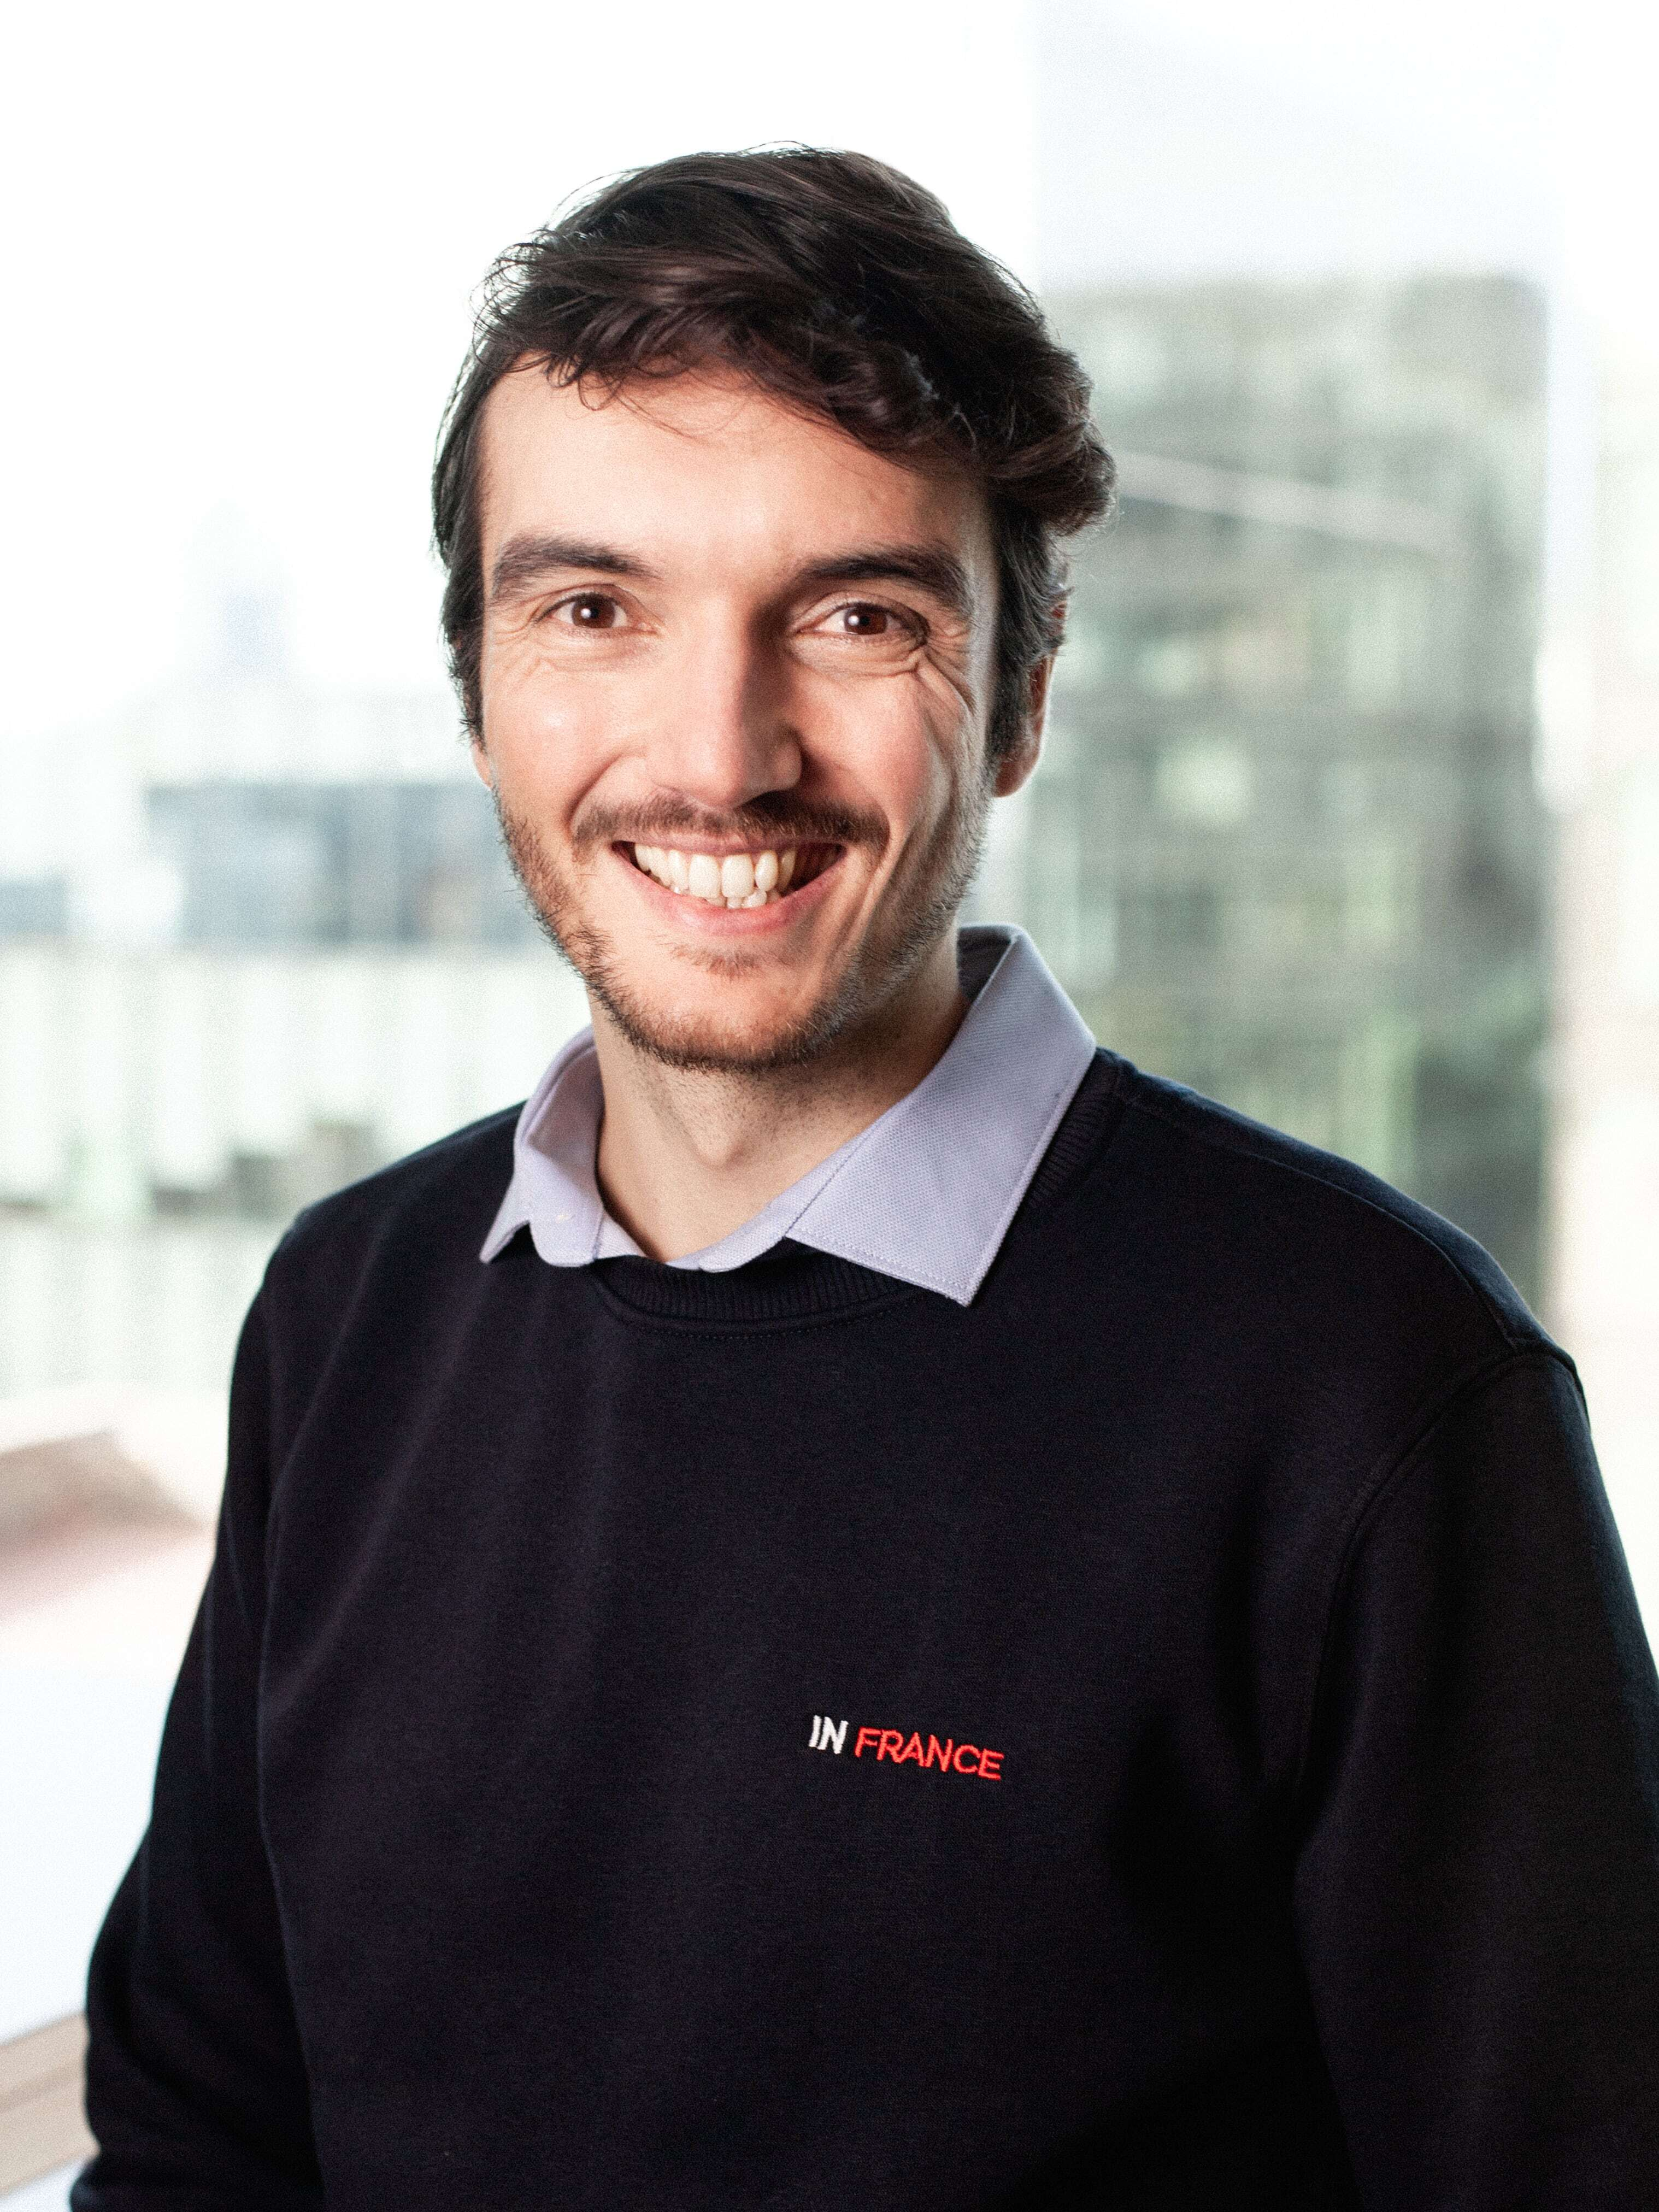
\includegraphics[width=5cm]{image/trombine-christophe}
        \end{columns}
    \end{frame}

    \subsection{Operating System}\label{subsec:os}

    \begin{frame}{Operating System}{Définition de l'OS\footnote{\label{os}C’est quoi un OS (O.S) ?, \url{https://culture-informatique.net/cest-quoi-un-os/}}}
        Un système d'exploitation (OS) est un ensemble de programmes qui gèrent les ressources matérielles et logicielles d'un ordinateur.
        Il permet également une interaction entre l'utilisateur et l'ordinateur.
        \begin{itemize}
            \item Gère le processeur, la mémoire, les périphériques.
            \item Fournit une interface utilisateur.
            \item Sert d'intermédiaire entre les logiciels et le matériel.
        \end{itemize}
        \bigbreak
        Sans OS, le hardware est inutilisable.
    \end{frame}

    \begin{frame}{Operating System}{Fonctionnement de l'OS\cref{os}}
        L'OS agit comme un intermédiaire entre les logiciels et le matériel.
        Les logiciels ne communiquent pas directement avec le matériel (ou très rarement autorisés par certains OS et sous certaines conditions), mais passent par l'OS~.
        \begin{itemize}
            \item Les logiciels sont installés sur l'OS~.
            \item Les logiciels sont compilés pour un OS spécifique (par exemple, un logiciel pour Windows ne fonctionnera pas sur IOS).
        \end{itemize}
    \end{frame}

    \begin{frame}{Operating System}{Les Pilotes (Drivers)\cref{os}}
        L'OS utilise des pilotes pour communiquer avec les périphériques.
        Un pilote est un programme qui agit comme un traducteur entre l'OS et le matériel.
        \begin{itemize}
            \item Chaque périphérique (souris, clavier, imprimante) a besoin d'un pilote pour fonctionner correctement.
            \item Exemple : le pilote d'une imprimante traduit les commandes de l'OS en instructions compréhensibles pour l'imprimante.
        \end{itemize}
    \end{frame}

    \begin{frame}{Operating System}{Évolution des OS\cref{os}}
        Historiquement, les premiers OS avaient une interface textuelle ou en ligne de commande, sans interface graphique.
        Quelques exemples d'OS historiques incluent :
        \begin{itemize}
            \item OS/360 d'IBM~.
            \item Unix.
            \item MSDOS.
            \item L'évolution vers des interfaces graphiques avec MacOS et Windows.
            \item Aujourd'hui, des OS comme Android dominent sur les smartphones.
        \end{itemize}
    \end{frame}

    \begin{frame}{Operating System}{Conclusion\cref{os}}
        L'OS est la colonne vertébrale de tout appareil informatique.
        Il gère les interactions entre les logiciels et le matériel, tout en offrant une interface pour l'utilisateur.
        Sans un OS, nos appareils modernes ne seraient que des coquilles vides incapables d'exécuter des tâches.
        \bigbreak
        \centering
        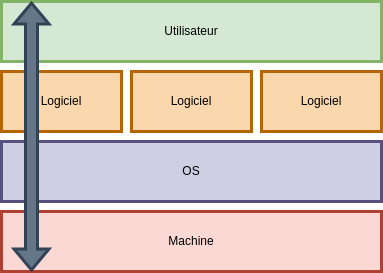
\includegraphics[width=7cm]{image/os.drawio}
    \end{frame}

    \subsection{Historique}\label{subsec:historique}

    \begin{frame}{Historique de Linux}{Linux, quelques caractéristiques de la première version\footnote{The early days of Linux, Lars Wirzenius, \url{https://lwn.net/Articles/928581/}}}
        \begin{footnotesize}
            \begin{itemize}
                \item La première version libérée par Linus Torvald, date de 1991 et sa licence ne permet pas l'usage commercial.
                \item Elle est compilée avec GCC 1.4, A.K.A. \textit{GNU C Compiler} de Richard Stallman.
                La publication de GCC en version 0.9 date de 1987.
                L.~Torvald a déjà porté GCC sous Minix, un OS éducatif\footnote{GCC,\url{https://gunkies.org/wiki/Gcc}}\footnotestep\footnote{A Brief Historu of GCC, \url{https://gcc.gnu.org/wiki/History}}.
                \item 1992, Linux est distribué sous license GNU GPL, donc pour tout usage, même commercial.
                \item 1992, intégration de X11, le serveur graphique, pour favoriser l'usage en \textit{desktop}.
                \item 1993, formation de la communauté Debian.
                \item Fin des années 90, les investissements d'IBM pour supporter Linux atteignent le milliard de dollars\footnote{A strong history and commitment to open source, \url{https://www.ibm.com/opensource/story/}}.
            \end{itemize}
        \end{footnotesize}
    \end{frame}

    \begin{frame}{Historique de Linux}{Historique de tous les OS\footnote{chococigar, \url{https://github.com/chococigar/cup-of-cs/blob/main/img/history\_of\_os.png}}}
        \centering
        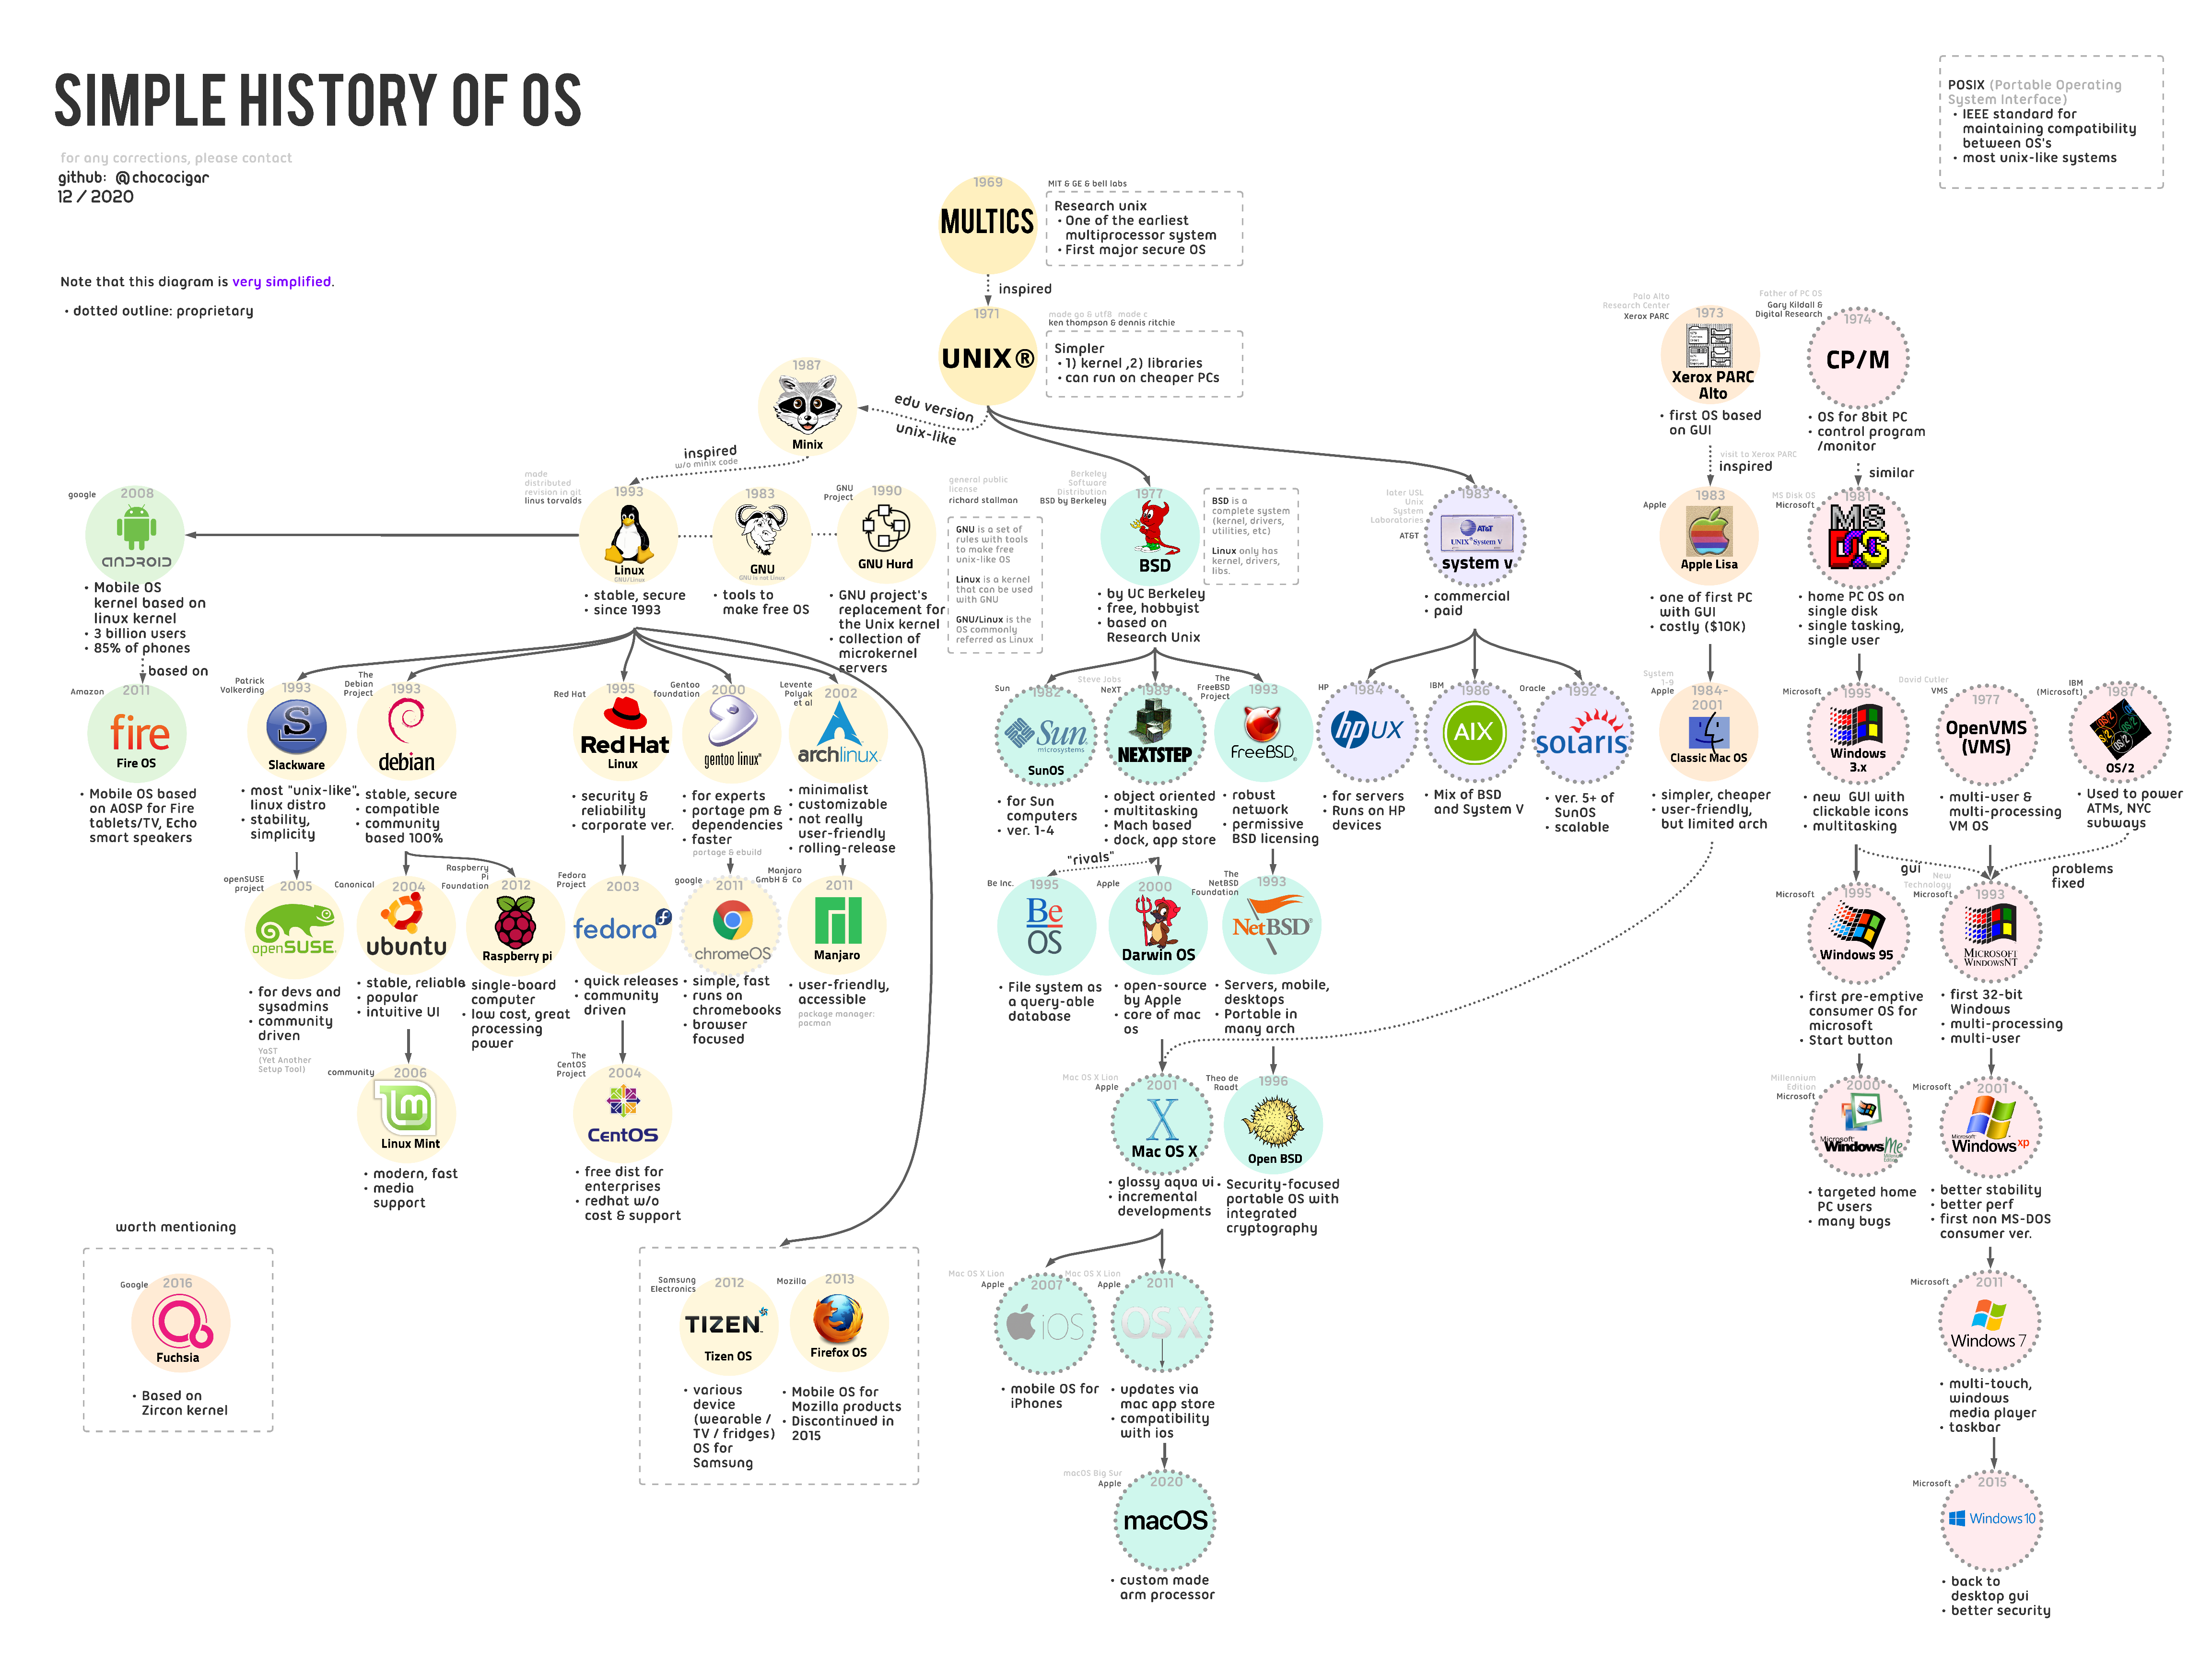
\includegraphics[width=9cm]{image/history_of_os}
    \end{frame}

    \begin{frame}{Historique de Linux}{Linux, historique des single/multi users OS}
        Multi user au sens \textit{Time-Sharing}, \textit{i.e.}, plus d'un utilisateur en même temps.

        Les premiers OS Multi user était OS/360 d'IBM dans les années 60.
        Un concurrent est développé par Bell Labs, une filiale d'AT\&T (Avant le démantèlement en 1982), c'est Unix en 1969.

        Linux est ainsi multi user dès le début.
        Par opposition à Windows, qui par défaut (sans RDP ni bricolage), ne l'est pas.
        C'est Windows® Server qui est multi user.
        \bigbreak
        Cette différence est cruciale, car elle a fait de cet OS un candidat idéal pour les serveurs (Web, BDD, \textit{etc}).
    \end{frame}

    \begin{frame}{Historique de Linux}{Adoption}
        \footnotetext{Why Linux runs 90 percent of the public cloud workload, \url{https://www.cbtnuggets.com/blog/certifications/open-source/why-linux-runs-90-percent-of-the-public-cloud-workload}}
        \footnotetext{\label{cbt}When everything is in the cloud, does the OS matter?, \url{https://www.redhat.com/en/blog/when-everything-cloud-does-os-matter}}
        \footnotetext{20 great years of Linux and supercomputer, \url{https://www.zdnet.com/article/20-great-years-of-linux-and-supercomputers/?ref=itsfoss.com}}
        \begin{columns}
            \column{0.5\textwidth}
            \begin{itemize}
                \item 2018, 90 \% des serveurs du cloud tournent sous Linux\footnotemark.
                \item 2018, 70 \% des serveurs sont déployés dans le cloud\footnotemark.
                \item 2018, 62 \% de l'embarqué\cref{cbt}.
                \item 2012, 95 \% des supercalculateurs\footnotemark.
            \end{itemize}
            \column{0.5\textwidth}
            \centering
            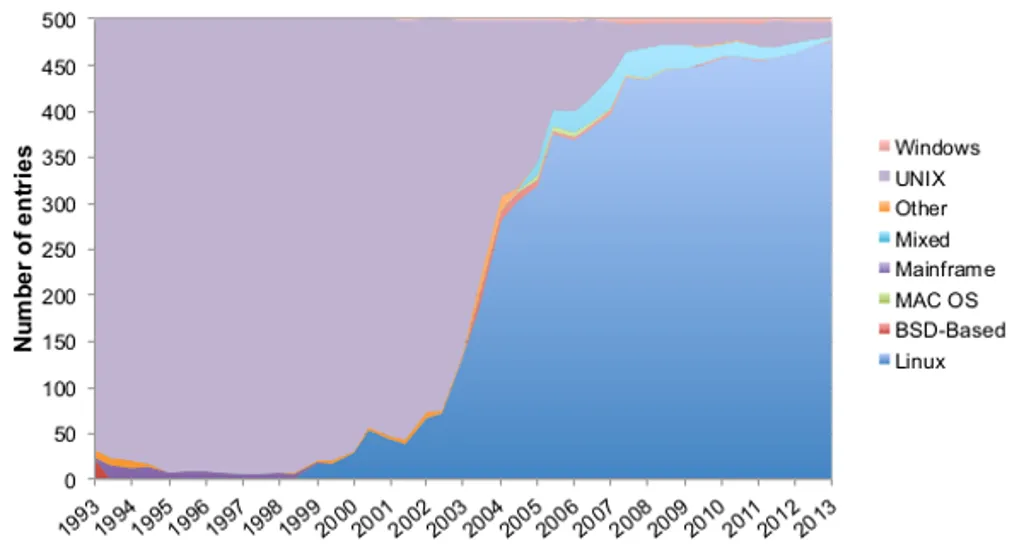
\includegraphics[width=6cm]{image/linux-supercomputer-growth}
        \end{columns}
    \end{frame}

    \subsection{Kernel et distribution}\label{subsec:kernel-et-distribution}

    \begin{frame}{Les distributions}{Définitions\footnote{Glossary, \url{https://help.ubuntu.com/community/Glossary}}}
        \begin{itemize}
            \item \textbf{Kernel} ou \textbf{Noyau}~: Le composant central d'un système d'exploitation qui contrôle tous les processus bas niveau d'un ordinateur, tels que la gestion de la mémoire, les threads et les entrées/sorties.
            En un sens, le noyau agit comme le gardien de l'ordinateur vis-à-vis du matériel.
            Les applications font des appels système via le noyau pour demander des ressources et interagir avec le matériel.
            \item \textbf{Distribution}~: Désigne une version de GNU/Linux ou d'un autre système d'exploitation open source, bien que certaines personnes soutiennent que le terme devrait inclure les différents systèmes d'exploitation Windows® et Apple.
            Ubuntu est la version la plus populaire, mais il en existe de nombreuses autres, telles que RedHat, qui est bien connue pour les serveurs.
            La plupart des autres distros sont conçues pour un type particulier d'architecture, comme les téléphones, les netbooks, les routeurs, les serveurs, \textit{etc}.
        \end{itemize}
    \end{frame}

    \begin{frame}{Kernel}{Définition\footnote{Linux fundamentals: user space, kernel space, and the syscalls API surface, \url{https://www.form3.tech/blog/engineering/linux-fundamentals-user-kernel-space}}}
        \centering
        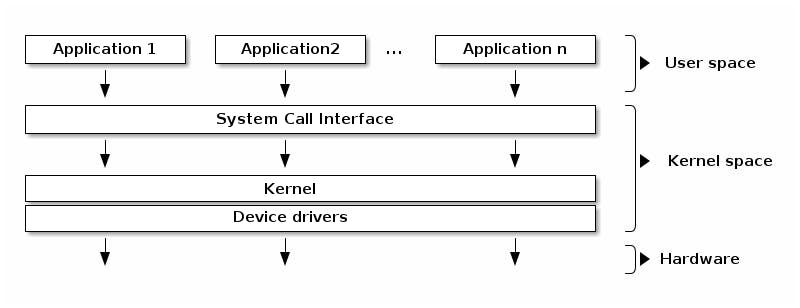
\includegraphics[width=10cm]{image/kernel}
        \flushleft
        \begin{itemize}
            \item \textbf{User space}~: L'espace utilisateur est l'endroit où les applications s'exécutent.
            \item \textbf{Kernel space}~: L'espace noyau est l'endroit où le noyau s'exécute.
            \item \textbf{Syscalls}~: Les appels système sont des interfaces entre les applications et le noyau.
        \end{itemize}
    \end{frame}

    \begin{frame}{Les distributions}{La timeline de toutes les distributions\footnote{FabioLolix, \url{https://github.com/FabioLolix/linuxtimeline}}\footnotestep\footnote{Put the fun back into computing. Use Linux, BSD., \url{https://distrowatch.com/}}}
        \begin{columns}
            \column{0.8\textwidth}
            Insights~:
            \begin{itemize}
                \item Les 3 plus grosses branches sont Debian, Red Hat et Ubuntu.
                \item Très nombreuses.
                \item Certaines branches meurent même après de longues années d'existence (Mandrake, Centos, \textit{etc}.).
                \item Certaines distributions passent d'une branche à l'autre.
            \end{itemize}
            Quid de l'impact sur la maintenance de la distribution~?
            \column{0.2\textwidth}
            \centering
            \includegraphics[width=1.5cm]{image/linux-all-distro-timeline}
        \end{columns}
    \end{frame}

    \begin{frame}{Les distributions}{La timeline de toutes les distributions}
        Red-Hat, filiale d'IBM, fait l'opposition entre les distributions \textit{entreprise} et les \textit{community}.
        En mettant en avant leur support de 10 ans contre 2 ans pour Fedora, une distribution communautaire de la même branche\footnote{What's the best Linux distro for you?, \url{https://www.redhat.com/en/topics/linux/whats-the-best-linux-distro-for-you}}.
        \bigbreak
        Ubuntu a un business model légèrement différent, ils proposent 5 ans de support pour les versions LTS et une extension de 10 ans dans la version payant appelée \textquote{Ubuntu Pro}\footnote{The Ubuntu lifecycle and release cadence, \url{https://ubuntu.com/about/release-cycle}}.
        \bigbreak
        Mais peut-être que l'exemple de Red-Hat n'est pas le bon, Debian, une distro communautaire également, communique un support des versions LTS de 5 ans minimum\footnote{Debian Long Term Support, \url{https://wiki.debian.org/LTS}}\ldots
    \end{frame}

    \begin{frame}{Les distributions}{La timeline des principales distributions\footnote{\label{main-distro}Philipp Leclercq, \url{https://github.com/PhilLecl/SanitizedLinuxTimeline}}}
        \centering
        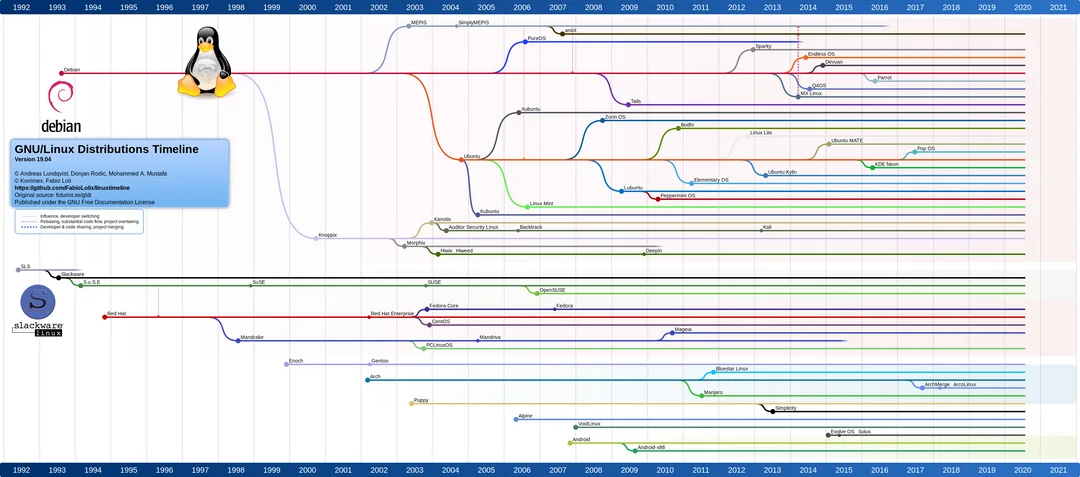
\includegraphics[width=12cm]{image/linux-main-distro-timeline}
    \end{frame}

    \begin{frame}{Les distributions}{Les licences des principales distributions\cref{main-distro}}
        \centering
        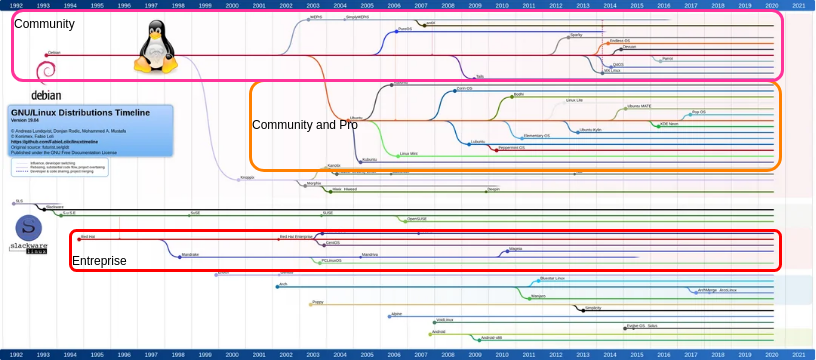
\includegraphics[width=12cm]{image/main-distro-license.drawio}
    \end{frame}

    \begin{frame}{Les distributions}{Les packages managers des principales distributions\cref{main-distro}}
        \centering
        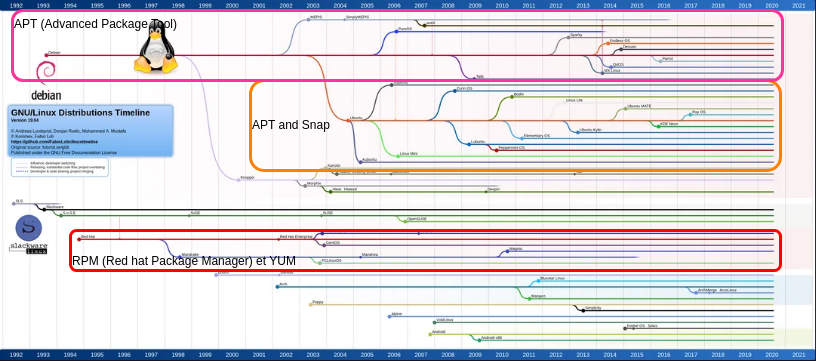
\includegraphics[width=12cm]{image/main-distro-package-manager.drawio}
    \end{frame}

    \begin{frame}{Les distributions}{Une aide pour choisir sa distribution}
        Le site Distrowatch propose un utilitaire pour trouver des distributions candidates en fonction d'un large nombre de critères, \url{https://distrowatch.com/search.php}.
        \bigbreak
        \centering
        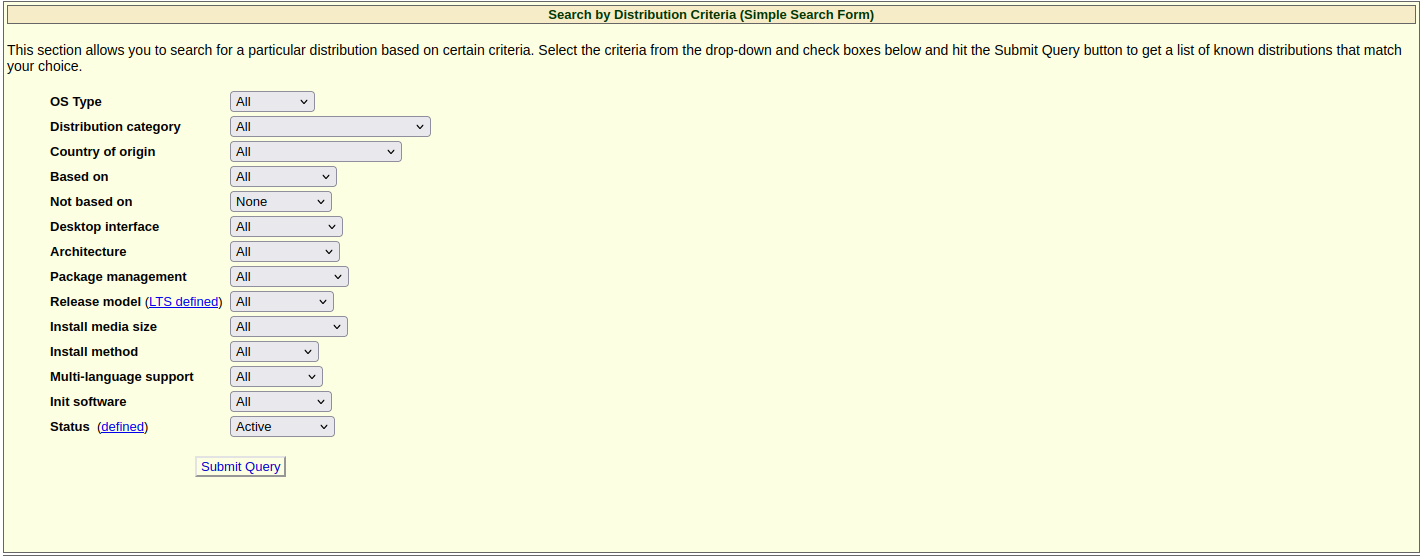
\includegraphics[width=12cm]{image/distrowatch-search}
    \end{frame}

    \begin{frame}{Les distributions}{Une aide pour choisir sa distribution}
        Admettons que tous les 2/3 packages managers mainstreams se valent.
        \bigbreak
        Un des critères différenciant, en plus du support que nous avons vu, est l'architecture.
        \bigbreak
        Qu'est-ce que le critère \textquote{architecture} et pourquoi est-ce important lors d'une migration~?
        \pause
        \bigbreak
        \begin{itemize}
            \item Une modernisation d'un hardware vieillissant qui peut être remplacé par une machine virtuelle faisant tourner les mêmes applications.
            \item Un hardware qui n'est plus supporté par la distribution actuelle et doit donc migrer.
        \end{itemize}
        Dans les 2 exemples, avoir une même architecture permettra ainsi une migration plus \textit{lean}.
        Sans rewrite, voire, sans recompilation.
    \end{frame}

    \begin{frame}{Les distributions}{Des critères manquants~?}
        Y-a-t-il des critères pertinents qui pourraient manquer~?
        \bigbreak
        \centering
        
\includegraphics[width=6cm]{image/question-mark}
    \end{frame}

    \begin{frame}{Les distributions}{Des critères manquants~?}
        L'énorme succès d'une distribution à part, Alpine Linux, pousser par les technologies de virtualisation et de conteneurisation.
        \bigbreak
        Une des premières phrases de présentation sur leur site est \textit{Alpine Linux is built around musl libc and busybox. A container requires no more than 8 MB and a minimal installation to disk requires around 130 MB of storage.}\footnote{About, \url{https://alpinelinux.org/about/}}.
        \bigbreak
        De leur analyse, qui est sûrement la bonne, leur succès vient du compilateur musl et de la librairie C libc musl.
    \end{frame}

    \begin{frame}{Les distributions}{Des critères manquants~?}
        Red-Hat recrute beaucoup d'experts de LLVM ces dernières années\footnote{Red Hat Is Hiring More LLVM Compiler Engineers, \url{https://www.phoronix.com/news/Red-Hat-More-LLVM-Engineers}}.

        Certaines distributions peuvent ou sont compilées avec LLVM comme FreeBSD\footnote{Building FreeBSD with clang/llvm, \url{https://wiki.freebsd.org/BuildingFreeBSDWithClang}}, Chimera\footnote{About Chimera Linux, \url{https://chimera-linux.org/about/}}, OpenMandriva\footnote{La communauté OpenMandriva annonce la disponibilité d'OpenMandriva Lx 4.0, \url{https://linux.developpez.com/actu/266344/La-communaute-OpenMandriva-annonce-la-disponibilite-d-OpenMandriva-Lx-4-0-qui-apporte-de-nombreuses-nouveautes-liees-a-LLVM-Clang/}}\ldots
    \end{frame}

    \begin{frame}{Les distributions}{Plusieurs combinaisons de compilateurs et libraries C}
        \centering
        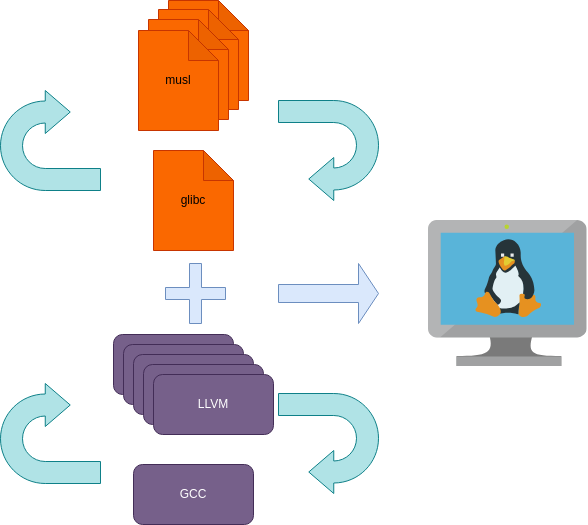
\includegraphics[width=8cm]{image/interchange-lib-compiler.drawio}
    \end{frame}

    \begin{frame}{Les distributions}{Conclusion}
        \begin{columns}
            \column{0.6\textwidth}
            Une distribution Linux est construite de manière modulaire~:
            \begin{itemize}
                \item Version de noyau.
                \item Packages manager.
                \item Architecture.
                \item Licence.
                \item Support.
                \item Librairie C~.
                \item Compilateur.
                \item \textit{Many more}.
            \end{itemize}
            \column{0.4\textwidth}
            \centering
            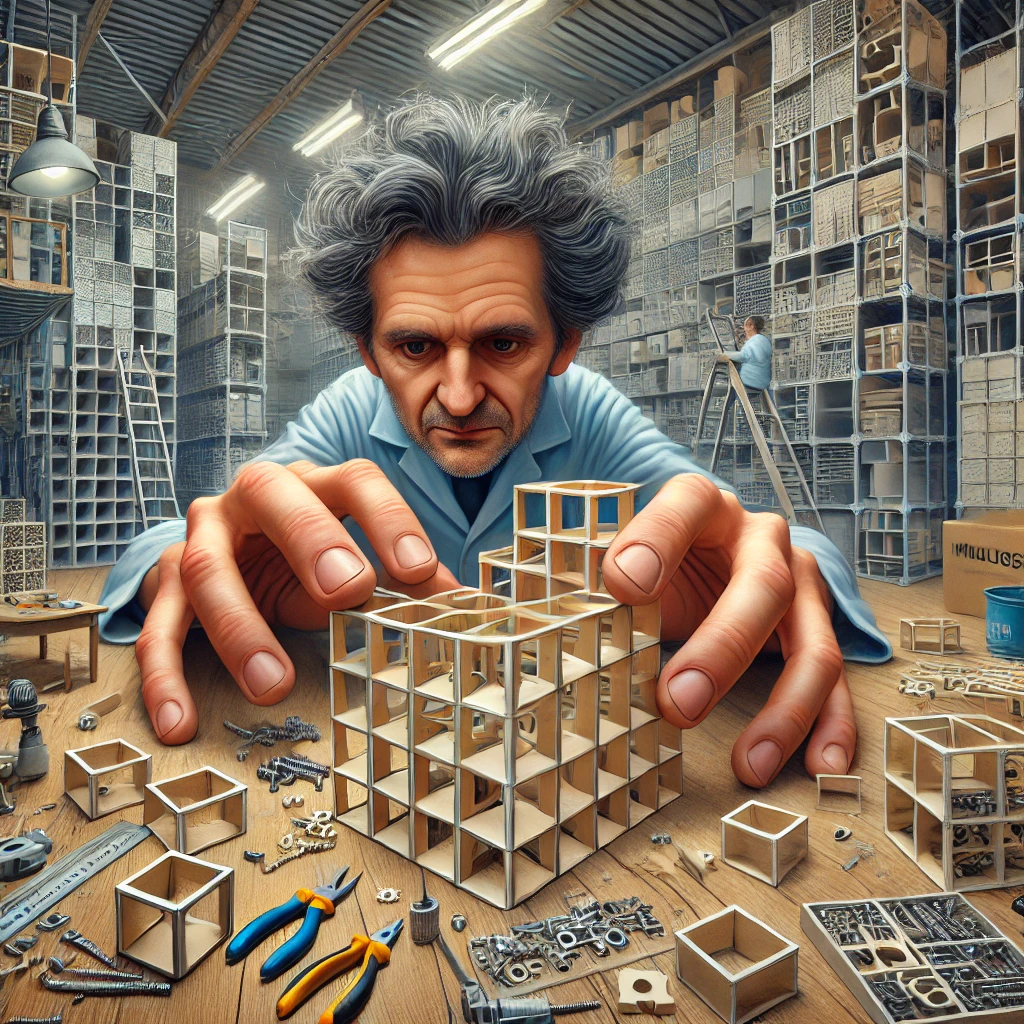
\includegraphics[width=5.5cm]{image/craftsman-focused}
        \end{columns}
        \bigbreak
        À vous de trouver la meilleure combinaison pour vos besoins.
    \end{frame}


    \section{Shell et commandes de base}\label{sec:shell-and-command}

    \subsection{Shell}\label{subsec:shell}

    \begin{frame}{Shell}{Qu'est-ce~?}
        Shell c'est~:
        \begin{itemize}
            \item C'est un exécutable.
            \item Un interpréteur de ligne de commande.
            Ne pas confondre avec des Shell spécifique comme le Python Shell ou le MySQL Shell qui interagissent spécifiquement avec ces applications.
            \item Et donc un interpréteur de scripts Shell.
            \item C'est une interface entre l'OS et l'humain.
            \item Existe sur la plupart des plateformes Linux, Unix, Windows® (\lstinline{Bash}, installé avec Git par exemple), \textit{etc}.
            \item Une portabilité poussée par une standardisation, comme la standardisation POSIX~.
            \item Des Shells plus \textit{user friendly} et plus lourds comme \lstinline{zsh}.
            \item Des Shells éxotiques comme \lstinline{tcsh} et \lstinline{csh}.
        \end{itemize}
    \end{frame}

    \begin{frame}{Shell}{Bourne Shell VS Bourne Again Shell\footnote{Difference between sh and bash, \url{https://www.geeksforgeeks.org/difference-between-sh-and-bash/}}}
        \begin{footnotesize}
            \begin{table}[h!]
                \centering
                \begin{tabular}{|p{5.5cm}|p{5.5cm}|}
                    \hline
                    \textbf{bash}                                     & \textbf{sh}                               \\ \hline
                    Bourne Again SHell                                & SHell                                     \\ \hline
                    Developed by Brain Fox                            & Developed by Stephen R. Bourne            \\ \hline
                    Successor of sh                                   & Predecessor of bash                       \\ \hline
                    bash is the default SHELL                         & sh is not the default SHELL               \\ \hline
                    \lstinline{\#\!/bin/bash}                         & \lstinline{\#\!/bin/sh}                   \\ \hline
                    It has more functionality with up-gradation       & It has less functionality                 \\ \hline
                    Supports job controls                             & Does not support job control              \\ \hline
                    bash is not a valid POSIX shell                   & sh is a valid POSIX shell                 \\ \hline
                    Easy to use                                       & Not as easy as bash                       \\ \hline
                    Less portable than sh                             & More portable than bash                   \\ \hline
                    Extended version of language                      & Original language                         \\ \hline
                    Bash scripting is scripting specifically for Bash & Shell scripting is scripting in any shell \\ \hline
                    Supports command history                          & Does not support command history          \\ \hline
                \end{tabular}
            \end{table}
        \end{footnotesize}
    \end{frame}

    \begin{frame}[fragile]{Shell}{Qu'est-ce~?}
        2 Shells sous une même distribution \textquote{légère} comme Alpine Linux~:
        \begin{lstlisting}[language=bash]
root@71641013d445:/usr/src/celia# sh
# ls
Dockerfile       README.pdf         UML-Sequence.drawio       celia.ipynb
# which sh
/usr/bin/sh
# which ls
/usr/bin/ls
# bash
root@71641013d445:/usr/src/celia# which bash
/usr/bin/bash
root@71641013d445:/usr/src/celia# which ls
/usr/bin/ls
root@71641013d445:/usr/src/celia# ls
Dockerfile       README.pdf         UML-Sequence.drawio       celia.ipynb
        \end{lstlisting}
        \bigbreak
        Comment interpréter ce code~?
    \end{frame}

    \begin{frame}{Shell}{Qu'est-ce~?}
        \begin{itemize}
            \item Un interpréteur de lignes de commandes.
            \item \lstinline{sh} et \lstinline{bash} appellent les mêmes exécutables.
            \item Shell n'est qu'une interface.
            \item Même dans une distribution \textquote{lightweight}, il y a 2 interpréteurs Shell~!
        \end{itemize}
        \bigbreak
        \lstinline{bash}, n'est pas installé par défault sur la dernière version de FreeBSD 14, uniquement \lstinline{sh}.
        Qu'en penser~?
        \bigbreak
        \centering
        
\includegraphics[width=3cm]{image/guy-in-front-of-desktop}
    \end{frame}

    \begin{frame}{Shell}{Bourne Shell VS Bourne Again Shell}
        Peut-on lister les avantages/inconvénients de l'un et l'autre~?
        \bigbreak
        \centering
        
\includegraphics[width=6cm]{image/question-mark}
    \end{frame}

    \begin{frame}{Shell}{Le poid de cette interface\footnote{Exigences matérielles pour utiliser Ubuntu, \url{https://doc.ubuntu-fr.org/exigences_minimales}}}
        Minimum 30 Go d'espace disque disponible pour une installation avec GNOME contre 5 Go ou 6 Go pour une installation Server ou Cloud.
        \bigbreak
        L'absence de bureau, avoir uniquement cette interface, est une des raisons de cette différence de taille.

        L'interface graphique n'est donc pas installé dans les distributions dédiées aux serveurs.
        Shell et l'accès Shell distant sécurisé \lstinline{SSH} (Secure SHell), sont utilisés.
        Un client SSH comme Putty, SSH de GitBASH sous Windows® ou un terminal sous Linux permettent d'accéder à un server Linux.
        \bigbreak
        GitBash permet d'unifier les deux environnements Linux et Windows, de pratiquer le Bash sur les 2 plateformes.
    \end{frame}

    \begin{frame}{Shell}{Pourquoi a-t-on un Shell ou l'autre~?}
        Quand je me connecte avec mon utilisateur, j'ai souvent \lstinline{bash} comme Shell.
        Pourquoi pas \lstinline{sh}~?
        \bigbreak
        \centering
        
\includegraphics[width=6cm]{image/question-mark}
    \end{frame}

    \begin{frame}[fragile]{Shell}{Pourquoi a-t-on un Shell ou l'autre~?}
        Probablement, l'administrateur système a créé votre utilisateur en spécifiant \lstinline{bash} comme Shell.
        \bigbreak
        Si on lit l'aide de la commande \lstinline{useradd}~:
        \begin{lstlisting}[language=bash]
$ useradd -h | grep shell
-s, --shell SHELL               interpréteur de commandes de connexion du nouveau compte
        \end{lstlisting}
        \bigbreak
        Un exemple de commande devient donc~:
        \begin{lstlisting}[language=bash]
$ useradd -s /bin/bash -m -d $/home/digiformateur digicomp
        \end{lstlisting}
        \bigbreak
        \lstinline{/bin/bash} passé à l'option \lstinline{-s} permet de spécifier le Shell.
    \end{frame}

    \begin{frame}{Shell}{Naviguer dans les commandes}
        \begin{itemize}
            \item \lstinline{history}~: Affiche l'historique des commandes.
            \item Ctrl+c~: Arrête l'exécution d'une commande.
            \item \emoji{up-arrow}~: Rappelle la dernière commande.
            \item \emoji{down-arrow}~: Rappelle la commande suivante.
            \item Ctrl+r~: Recherche dans l'historique des commandes.
            \item \lstinline{\\}~: Permet de continuer une commande sur la ligne d'après.
            \item \lstinline{\&}~: Lancer une commande en arrière-plan.
            \item Ctrl+z~: Mettre une commande en pause.
            \item \lstinline{fg}~: Reprendre une commande en pause.
            \item \lstinline{bg}~: Reprendre une commande en pause en arrière-plan.
        \end{itemize}
    \end{frame}

    \begin{frame}{Shell}{Gérer plusieurs commandes en parallèle avec \lstinline{tmux}\footnote{\label{itm:tmux}Tmux (terminal multiplexer), \url{https://www.redhat.com/sysadmin/introduction-tmux-linux}}}
        \lstinline{tmux} est un multiplexeur de terminal, \textit{i.e.}, permet d'ouvrir plusieurs fenêtres dans un terminal.
        Chacune faisant tourner un processus.
        \begin{footnotesize}
            \begin{table}[ht]
                \centering
                \begin{tabular}{|p{3.5cm}|p{8cm}|}
                    \hline
                    \textbf{Commande}         & \textbf{Description}                                                            \\
                    \hline
                    Ctrl+b puis D             & Détacher de la session courante                                                 \\
                    \hline
                    Ctrl+b puis \%            & Diviser la fenêtre en deux volets horizontalement                               \\
                    \hline
                    Ctrl+b puis ``            & Diviser la fenêtre en deux volets verticalement                                 \\
                    \hline
                    Ctrl+b puis Flèche        & Se déplacer entre les volets                                                    \\
                    \hline
                    Ctrl+b puis X             & Fermer le volet                                                                 \\
                    \hline
                    Ctrl+b puis C             & Créer une nouvelle fenêtre                                                      \\
                    \hline
                    Ctrl+b puis N ou P        & Passer à la fenêtre suivante ou précédente                                      \\
                    \hline
                    Ctrl+b puis 0 (1,2\ldots) & Aller à une fenêtre spécifique par numéro                                       \\
                    \hline
                    Ctrl+b puis~:             & Entrer dans la ligne de commande pour taper des commandes (avec autocomplétion) \\
                    \hline
                    Ctrl+b puis ?             & Voir tous les raccourcis clavier (appuyer sur Q pour quitter)                   \\
                    \hline
                    Ctrl+b puis W             & Ouvrir un panneau pour naviguer entre les fenêtres de plusieurs sessions        \\
                    \hline
                \end{tabular}
            \end{table}
        \end{footnotesize}
    \end{frame}

    \begin{frame}{Shell}{Gérer plusieurs commandes en parallèle avec \lstinline{tmux}\cref{itm:tmux}}
        Par exemple pour monitorer les ressources avec \lstinline{top} dans le terminal de droite, pendant qu'on lance la commande dans celui de gauche.
        \bigbreak
        \centering
        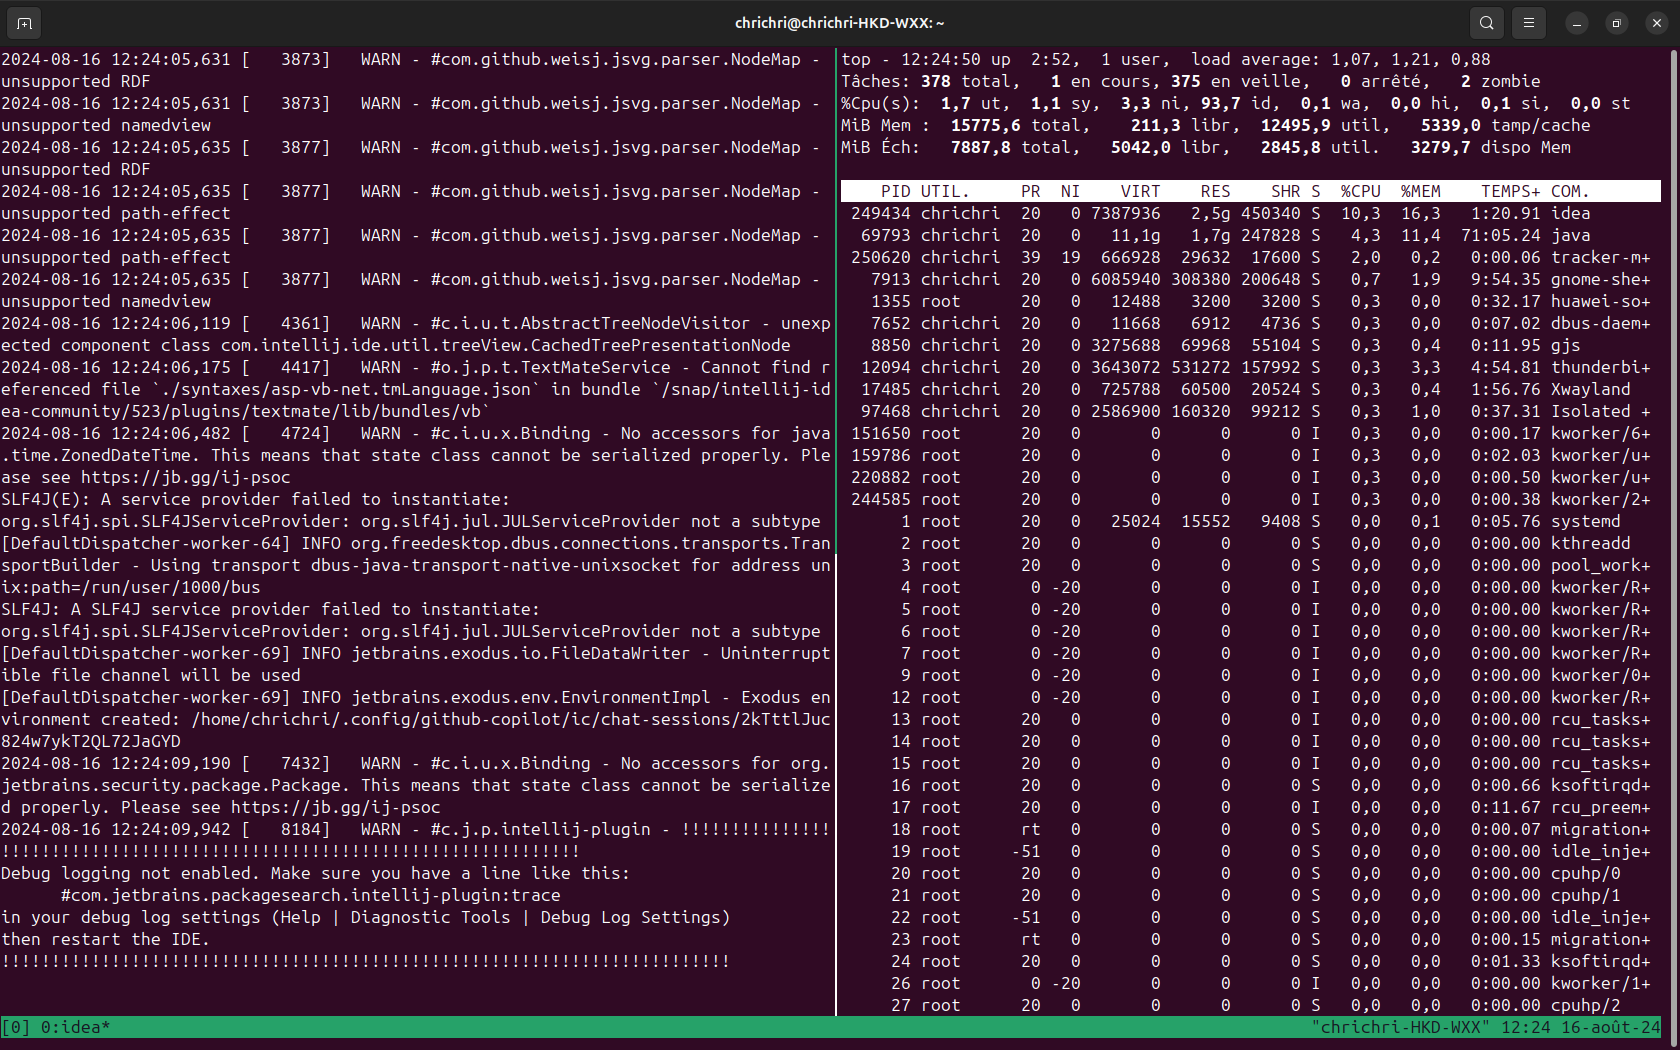
\includegraphics[width=10.3cm]{image/tmux-illustration}
    \end{frame}

    \begin{frame}[fragile]{Shell}{Gérer plusieurs commandes en parallèle avec \lstinline{nohup}}
        \lstinline{nohup} vient de NO Hang UP, c'est une commande qui permet de lancer une autre commande en arrière-plan sans qu'elle soit interrompue par la fermeture de la session Shell.
        Idéale donc pour les longs processus.
        L'output de la commande va par défault dans le fichier \lstinline{nohup.out}.
        \bigbreak
        Il suffit de préfixer la commande par \lstinline{nohup} et d'ajouter un \lstinline{&} pour libérer le terminal.
        \lstinline{nohup} indique le PID pour pouvoir stopper la commande au besoin et indique également quand la commande est terminée, si elle s'est arrêtée (Termine <code retour>) prématurément ou normalement (Fini).
        \begin{lstlisting}[language=bash]
$ nohup ls &
[1] 279343
nohup: les entrées sont ignorées et la sortie est ajoutée à 'nohup.out'
[1]+  Fini                    nohup ls
$ tail -n 3 nohup.out
technip
Téléchargements
ts-test
        \end{lstlisting}
    \end{frame}

    \begin{frame}[fragile]{Shell}{Les allias}
        Les allias sont des raccourcis pour des commandes.
        ils sont donc intéressant à paramétrer pour les commandes longues et récurrente.
        \bigbreak
        Par exemple, pour la commande \lstinline{ls -l}~:
        \begin{lstlisting}[language=bash]
$ alias ll='ls -l'
$ ll
total 3484
-rw-rw-r-- 1 chrichri chrichri     249 août  15 12:35 analytic-using-awk.sh
-rw-rw-r-- 1 chrichri chrichri      82 août  10 23:04 checkmytex.sh
...
        \end{lstlisting}
        \bigbreak
        Pour rendre l'allias permanent, il faut l'ajouter dans le fichier \lstinline{.bashrc} ou \lstinline{.bash\_profile}~:
        \begin{lstlisting}[language=bash]
$ echo "alias ll='ls -l'" >> ~/.bashrc
        \end{lstlisting}
        De cette manière à chaque fois qu'un Shell est ouvert, la commande est exécutée.
    \end{frame}

    \begin{frame}{Shell}{Secure SHell (SSH)}
        La machine Linux à administrer sera le plus souvent dans un cloud, une salle serveur, un data center, elle sera distante.
        Dans une infrastructure sécurisée.
        \bigbreak
        Mais avec un user, un Shell par défaut, et un protocole sécurisé comme le SSH~.
        Nous allons pouvoir nous connecter et l'administrer à distance.
        \bigbreak
        Les bonnes pratiques sont d'utiliser les clés SSH uniquement, pas de connexion SSH avec l'utilisateur root,
        Tutoriel utile~:
        \begin{itemize}
            \item \href{https://phoenixnap.com/kb/generate-setup-ssh-key-ubuntu}{Configuration du login SSH sur Ubuntu}
        \end{itemize}
        \bigbreak
        \centering
        
\includegraphics[width=3cm]{image/guy-in-front-of-desktop}
    \end{frame}

    \begin{frame}{Shell}{Sécurisation du SSH avec la cryptographie asymétrique}
        \begin{small}
            Pourquoi est-ce plus sécure d'utiliser une clé SSH plutôt qu'un mot de passe~?
            \bigbreak
            Quels algorithmes et taille de clés sont recommandés~?
            \pause
            \bigbreak
            Sur le site \url{https://jadaptive.com/ssh-key-management/the-benefits-of-ssh-key-authentication/} on trouve~:
            \begin{columns}
                \begin{column}{0.6\textwidth}
                    \begin{itemize}
                        \item Le mot de passe doit être communiqué à chaque connexion, il est donc plus vulnérable à une interception/sniffing/MITHM~.
                        La clé privée reste sur le client, elle n'est pas communiquée.
                        \item La clé SSH est plus complexe à deviner qu'un mot de passe.
                        \item On peut automatiser des taches depuis la machine cliente avec la clé SSH~.
                    \end{itemize}
                \end{column}
                \begin{column}{0.4\textwidth}
                    \centering
                    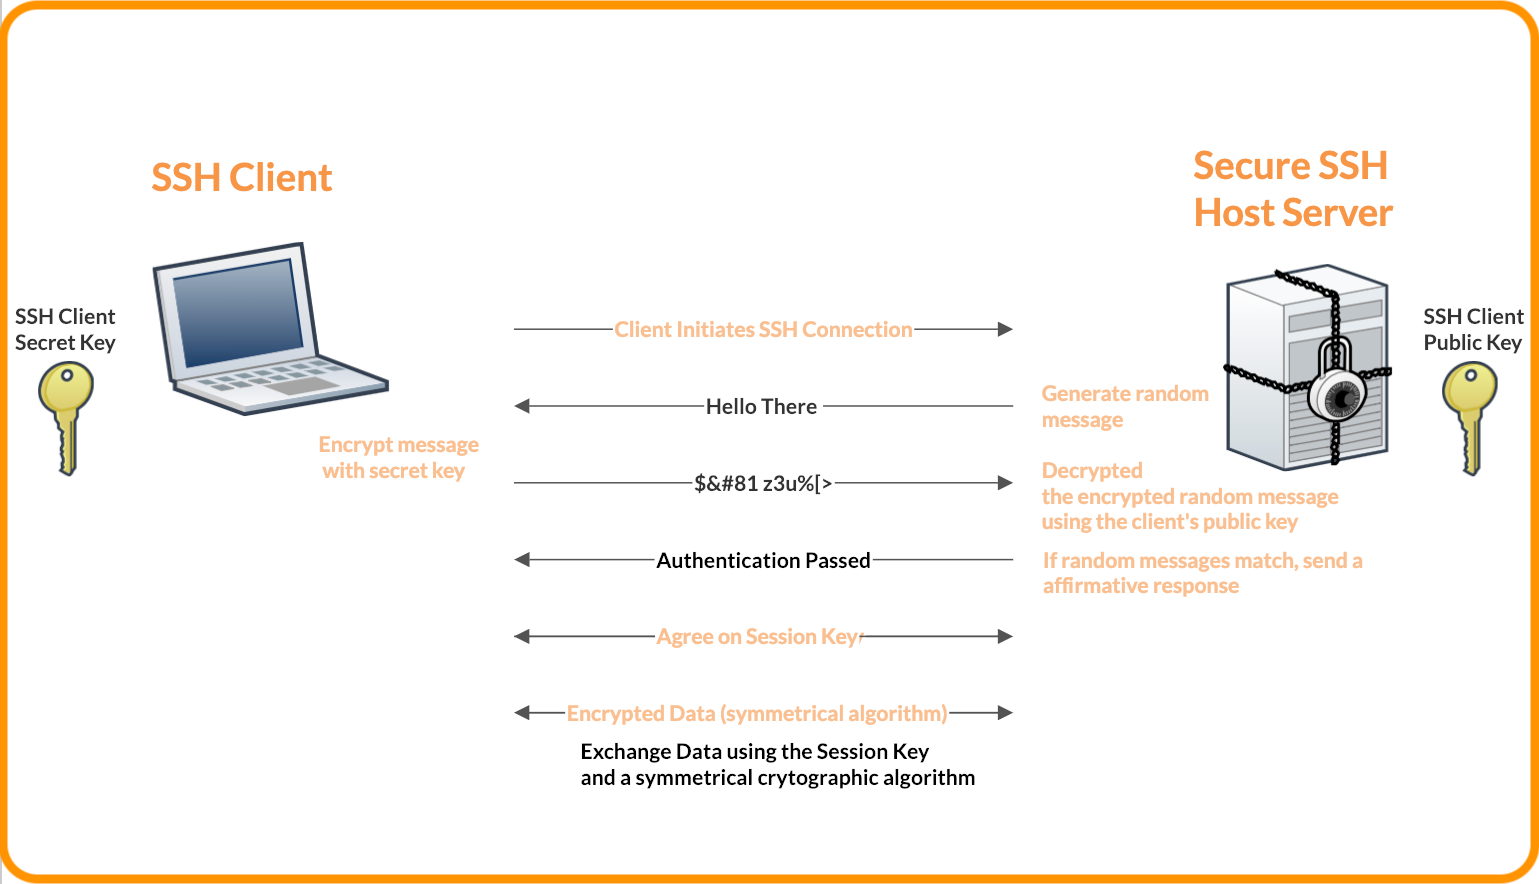
\includegraphics[width=5cm]{image/ssh-key-diagram} \\ Foxpass\footnotemark \\
                \end{column}
            \end{columns}
        \end{small}
    \end{frame}

    \begin{frame}{Shell}{Sécurisation du SSH avec la cryptographie asymétrique}
        Exercice \execcounterdispinc{}~:
        Restreindre l'accès à la VM au SSH avec une clé SSH, aucun mot de passe.
        \bigbreak
        Exercice \execcounterdispinc{}~:
        Créer un user pour un de vos camarades.
        Lui donner un Shell \lstinline{sh} par défaut.
        Configurer lui communiquer les clés SSH pour qu'il puisse se connecter.
    \end{frame}

    \begin{frame}[fragile]{Shell}{Une des solutions (commande à exécuter sur la VM)}
        Commande pour configurer la VM~:
        \begin{lstlisting}[language=bash][fragile]
# Configure SSH
sudo sed -i 's/PermitRootLogin yes/PermitRootLogin no/' /etc/ssh/sshd_config
sudo sed -i 's/PasswordAuthentication yes/PasswordAuthentication no/' /etc/ssh/sshd_config
# Restart SSH with the new configuration
sudo systemctl restart sshd
# Create the .ssh directory and the authorized_keys file
mkdir -p ~/.ssh
touch ~/.ssh/authorized_keys
# Add the public key to the authorized_keys file
echo "ssh-rsa AAAAB3NzaC1yc2EAAAADAQABAAABgQDQ8z4... chrichri@localhost" >> ~/.ssh/authorized_keys
        \end{lstlisting}
        \begin{center}
            
\includegraphics[width=2cm]{image/digicomp-lightbulb} \\ Expliquer chaque commande \\
        \end{center}
    \end{frame}

    \begin{frame}[fragile]{Shell}{Exemple de sécurisation des clés et des secrets sous Linux}
        Par défaut, Ubuntu desktop s’installe sur une partition non
        chiffrée (encrypter, ce n’est pas français on dit chiffrer~!~).
        Tout document peut donc être lu avec un disque de
        démarrage (live CD, USB bootable, \textit{etc}) ou si le disque dur
        est extrait et lu (vol, perte du desktop\ldots).
        \bigbreak
        Avec le package \lstinline{ecryptfs-utils} on peut chiffrer une partition~:
        \begin{lstlisting}[language=bash]
$ sudo apt-get install ecryptfs-utils
$ ecryptfs-setup-private
$ cp -r .ssh/ Private/ # Pour proteger les clés SSH on les déplace
$ ln -s /home/<mon user Ubuntu>/Private/.ssh/ . # Lien symbolique
        \end{lstlisting}
        Output~:
        \begin{lstlisting}
$ ls ~/.ssh -d -lha
lrwxrwxrwx 1 chrichri chrichri 28 janv. 14 21:27 /home/chrichri/.ssh -> /home/chrichri/Private/.ssh/
        \end{lstlisting}
        Il utilise le mot de passe de la session pour chiffrer/déchiffrer.
        Si la session n'est pas ouverte, les données sont chiffrées.
    \end{frame}

    \subsection{Commandes de base}\label{subsec:commandes-de-base}

    \begin{frame}{Commandes de base}{Commandes de base}
        \begin{itemize}
            \item \lstinline{ls}~: Liste les fichiers et répertoires.
            \item \lstinline{cd}~: Change de répertoire.
            \item \lstinline{pwd}~: Affiche le répertoire courant.
            \item \lstinline{cp}~: Copie des fichiers et des répertoires.
            \item \lstinline{mv}~: Déplace des fichiers et des répertoires.
            \item \lstinline{rm}~: Supprime des fichiers et des répertoires.
            \item \lstinline{mkdir}~: Crée des répertoires.
            \item \lstinline{cat}~: Affiche le contenu d'un fichier.
            \item \lstinline{head}~: Affiche les premières lignes d'un fichier.
            \item \lstinline{tail}~: Affiche les dernières lignes d'un fichier.
            \item \lstinline{touch}~: Crée un fichier vide.
            \item \lstinline{echo}~: Affiche une chaîne de caractères.
            \item \lstinline{du}~: Affiche l'espace disque utilisé par les fichiers.
            \item \lstinline{wget}~: Télécharge un fichier depuis URL~.
        \end{itemize}
    \end{frame}

    \begin{frame}[fragile]{Commandes de base}{Les options}
        Mais souvent, une commande seule ne suffit pas, il faut utiliser des options.

        Il existe deux solutions pour découvrir ces options~:
        \begin{itemize}
            \item Utiliser l'aide de la commande.
            Le plus souvent avec l'option \lstinline{-h}, équivalente à \lstinline{--help}.
            \begin{lstlisting}[language=bash]
$ ls --help # -h c'est human readable avec ls...
            \end{lstlisting}
            \item Ce qui revient à lire la documentation de la commande avec la commande~:
            \begin{lstlisting}[language=bash]
$ man ls # Same as above
            \end{lstlisting}
        \end{itemize}
    \end{frame}

    \begin{frame}[fragile]{Commandes de base}{Busy box}
        BusyBox est un logiciel libre qui fournit une implémentation unique d'environ 200 commandes UNIX standards dans un seul fichier pour diminuer la taille de ces derniers.
        Des distributions comme Alpine Linux l'utilisent pour réduire la taille de l'OS~.
        \begin{lstlisting}[language=bash,basicstyle=\tiny\ttfamily]
$ busybox
BusyBox v1.36.1 (Ubuntu 1:1.36.1-6ubuntu3) multi-call binary.
BusyBox is copyrighted by many authors between 1998-2015.
Licensed under GPLv2. See source distribution for detailed
copyright notices.

Usage: busybox [function [arguments]...]
or: busybox --list[-full]
or: busybox --install [-s] [DIR]
or: function [arguments]...

BusyBox is a multi-call binary that combines many common Unix
utilities into a single executable.  The shell in this build
is configured to run built-in utilities without $PATH search.
You don't need to install a link to busybox for each utility.
To run external program, use full path (/sbin/ip instead of ip).

Currently defined functions:
[, [[, acpid, adjtimex, ar, arch, arp, arping, ascii, ash, awk, base64, basename, bc, blkdiscard, blockdev, brctl, bunzip2, busybox, bzcat, bzip2, cal, cat, chgrp, chmod, chown, chpasswd, chroot, chvt, clear, cmp, cp,
cpio, crc32, crond, crontab, cttyhack, cut, date, dc, dd, deallocvt, depmod, devmem, df, diff, dirname, dmesg, dnsdomainname, dos2unix, dpkg, dpkg-deb, du, dumpkmap, dumpleases, echo, ed,
        \end{lstlisting}
    \end{frame}
    \begin{frame}[fragile]{Commandes de base}{Busy box}
        \begin{lstlisting}[language=bash,basicstyle=\tiny\ttfamily]
egrep, env, expand, expr, factor,
fallocate, false, fatattr, fdisk, fgrep, find, findfs, fold, free, freeramdisk, fsfreeze, fstrim, ftpget, ftpput, getopt, getty, grep, groups, gunzip, gzip, halt, head, hexdump, hostid, hostname, httpd, hwclock, i2cdetect,
i2cdump, i2cget, i2cset, i2ctransfer, id, ifconfig, ifdown, ifup, init, insmod, ionice, ip, ipcalc, kill, killall, klogd, last, less, link, linux32, linux64, linuxrc, ln, loadfont, loadkmap, logger, login, logname,
logread, losetup, ls, lsmod, lsscsi, lzcat, lzma, lzop, md5sum, mdev, microcom, mim, mkdir, mkdosfs, mke2fs, mkfifo, mknod, mkpasswd, mkswap, mktemp, modinfo, modprobe, more, mount, mt, mv, nameif, nbd-client, nc, netstat,
nl, nologin, nproc, nsenter, nslookup, nuke, od, openvt, partprobe, passwd, paste, patch, pidof, ping, ping6, pivot_root, poweroff, printf, ps, pwd, rdate, readlink, realpath, reboot, renice, reset, resume, rev, rm, rmdir,
rmmod, route, rpm, rpm2cpio, run-init, run-parts, sed, seq, setkeycodes, setpriv, setsid, sh, sha1sum, sha256sum, sha3sum, sha512sum, shred, shuf, sleep, sort, ssl_client, start-stop-daemon, stat, static-sh, strings, stty,
su, sulogin, svc, svok, swapoff, swapon, switch_root, sync, sysctl, syslogd, tac, tail, tar, taskset, tc, tee, telnet, telnetd, test, tftp, time, timeout, top, touch, tr, traceroute, traceroute6, true, truncate, ts, tty,
tunctl, ubirename, udhcpc, udhcpc6, udhcpd, uevent, umount, uname, uncompress, unexpand, uniq, unix2dos, unlink, unlzma, unshare, unxz, unzip, uptime, usleep, uudecode, uuencode, vconfig, vi, w, watch, watchdog, wc, wget,
which, who, whoami, xargs, xxd, xz, xzcat, yes, zcat
$ busybox ls
LICENSE            checkmytex.sh      compress-image.sh  dept.csv           employee.csv       sqlite-hr.sh       venv
        \end{lstlisting}
        Et s'utilise en préfixant la commande par \lstinline{busybox <commande>}.
        \begin{lstlisting}[language=bash,basicstyle=\tiny\ttfamily]
$ busybox sha256sum employee.csv
c148c36111463e962f490742af787c1f8e49776f09d89e19f71c6cdcf220240d  employee.csv
        \end{lstlisting}
    \end{frame}

    \begin{frame}{Commandes de base}{Exercice \execcounterdispinc{}~:}
        Le but est de préparer la configuration d'un nouveau service après avoir sauvegardé l'original.
        \begin{itemize}
            \item Créer un répertoire de backup des services dans votre \textquote{home} nommé \lstinline{service-backup}.
            \item Se déplacer dans le répertoire des services \lstinline{/etc/systemd/system}.
            \item Copier un service dans \lstinline{service-backup}.
            \item Afficher le contenu du fichier copié pour vérifier ce dernier.
            \item Créer un répertoire de développement des services dans votre \textquote{home} nommé \lstinline{service-dev}.
            \item Copier le contenu de \lstinline{service-backup} dans \lstinline{service-dev}.
            \item Modifier la description du service de \lstinline{service-dev} avec un éditeur et sauvegarder.
        \end{itemize}
    \end{frame}

    \begin{frame}{Commandes de base}{Opérateurs de redirection et piping\footnote{Five ways to use redirect operators in Bash, \url{https://www.redhat.com/sysadmin/redirect-operators-bash}}}
        \begin{itemize}
            \item \lstinline{>}~: Redirige la sortie standard vers un fichier.
            \item \lstinline{>>}~: Redirige la sortie standard vers un fichier en ajoutant le contenu à la fin.
            \item \lstinline{<}~: Redirige un fichier vers l'entrée standard.
            \item \lstinline{2>}~: Redirige la sortie d'erreur vers un fichier.
            \item \lstinline{|}~: Piping, redirige la sortie standard d'une commande vers l'entrée standard d'une autre.
        \end{itemize}
        À quoi ces opérateurs peuvent-ils servir~?
        \begin{center}
            
\includegraphics[width=2.5cm]{image/question-mark}
        \end{center}
    \end{frame}

    \begin{frame}{Commandes de base}{Exercice \execcounterdispinc{}~:}
        Le but est de créer un fichier source d'un script Shell en y ajoutant ligne par ligne les commandes~:
        \begin{itemize}
            \item Initier la création d'un script Shell nommé \lstinline{discover.sh} dans votre \textquote{home} avec un commentaire descriptif.
            \item Afficher un message indiquant que le \textquote{current working directory} va s'afficher.
            \item Afficher le \textquote{current working directory}.
            \item Afficher un message indiquant que les fichiers et répertoires du répertoire courant vont s'afficher.
            \item Afficher la liste des fichiers et répertoires du répertoire courant.
        \end{itemize}

        Inutile donc indispensable~:
        \begin{itemize}
            \item Changer de répertoire pour aller dans le répertoire courant avec le pipe.
        \end{itemize}
    \end{frame}


    \section{Licence CC}\label{sec:licence}

    \begin{frame}{Licence}{Licence Creative Commons}
        Support de cours sous licence Creative Commons BY-NC-ND~.
        \bigbreak
        Vous pouvez donc, partager, copier, distribuer le document.
        \bigbreak
        Attribution requise à PapIT SASU - Pas d’utilisation commerciale - Pas de modification
        \bigbreak
        \centering
        
\includegraphics[width=5cm]{image/by-nc-nd-logo}
    \end{frame}


\end{document}
